\begin{landscape}
\subsection{Zeit}	
    \begin{figure}[h!]
        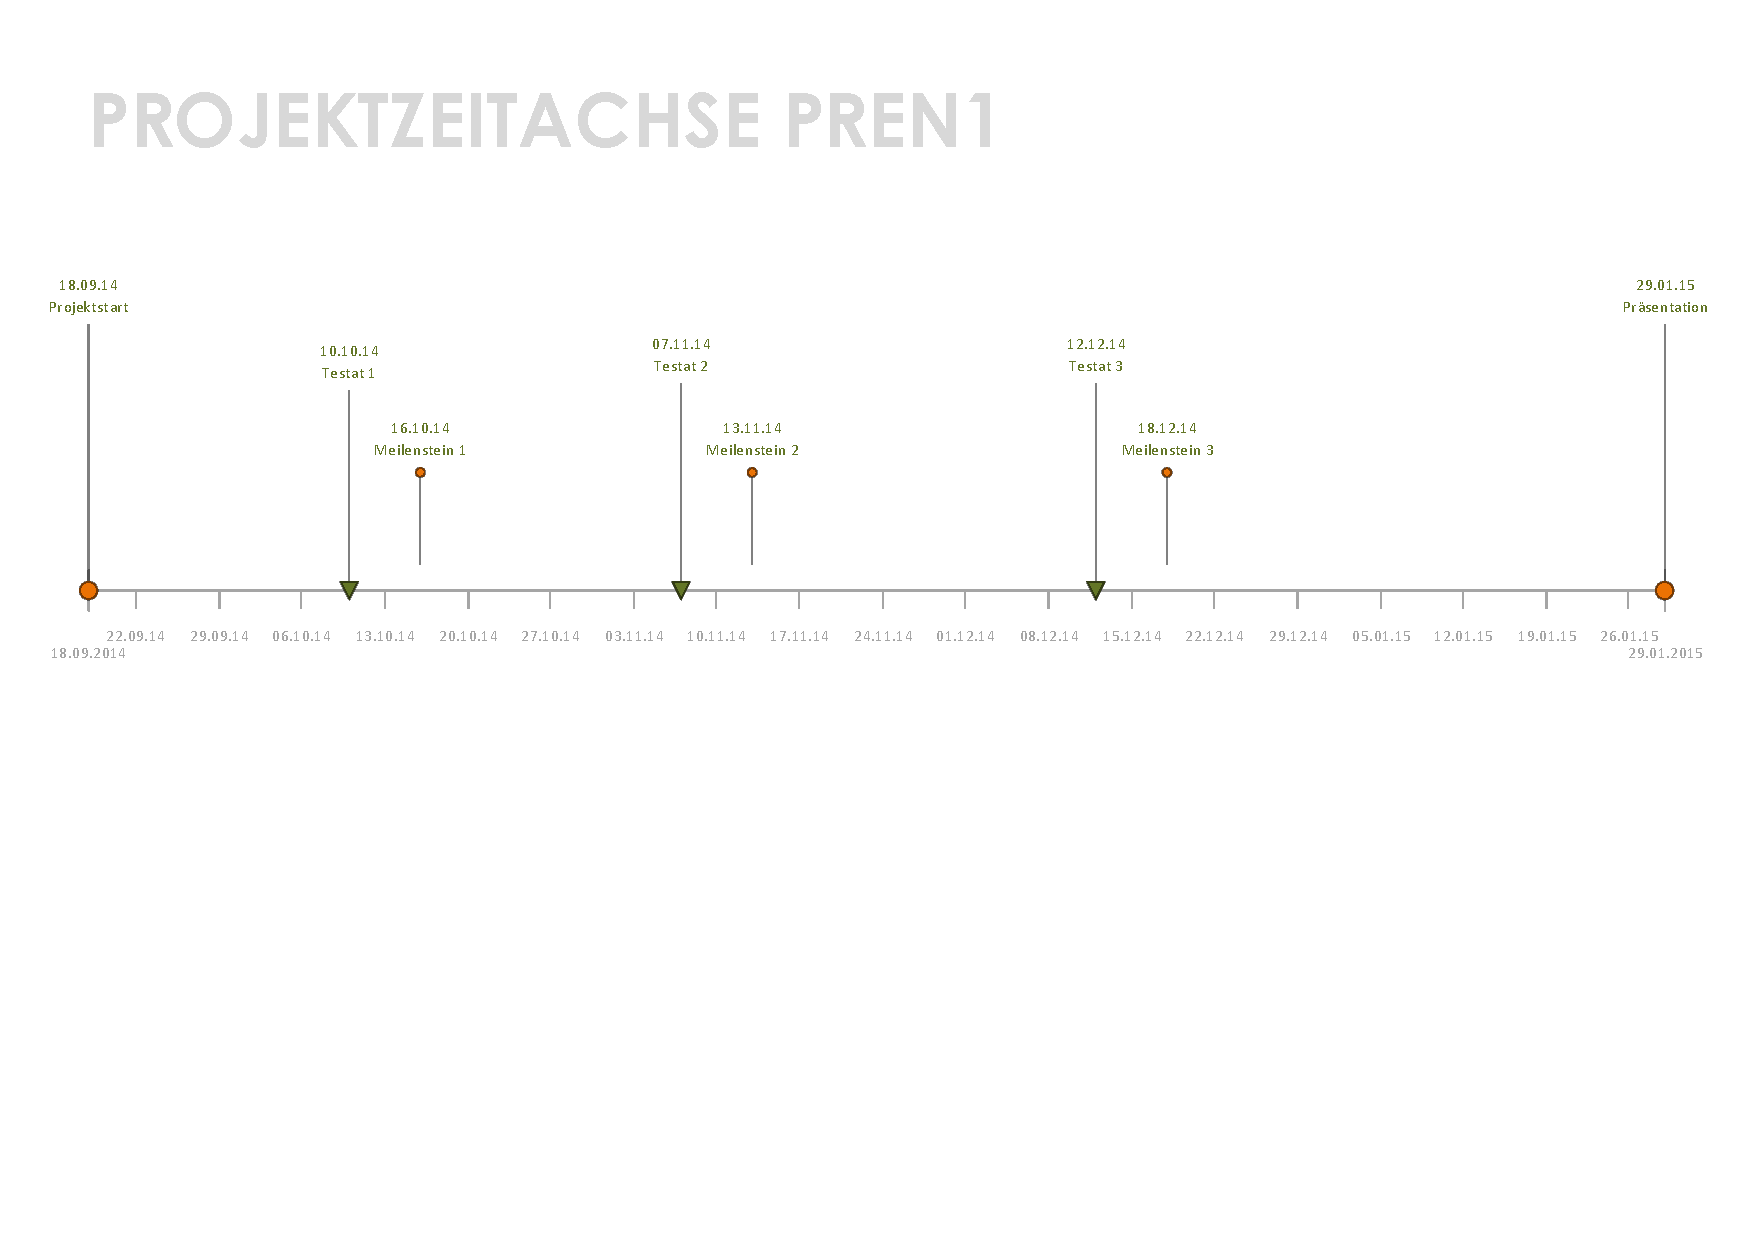
\includegraphics[page=1,scale=0.8,clip,trim=7mm 90mm 31mm 39mm] {Enddokumentation/Projektplanung_Management/Bilder/Projektzeitachse.pdf}
        \centering
        \caption{Zeitplan des Projekts} 
        \label{abb:ProjektZeitstrahl}
    \end{figure}
    
    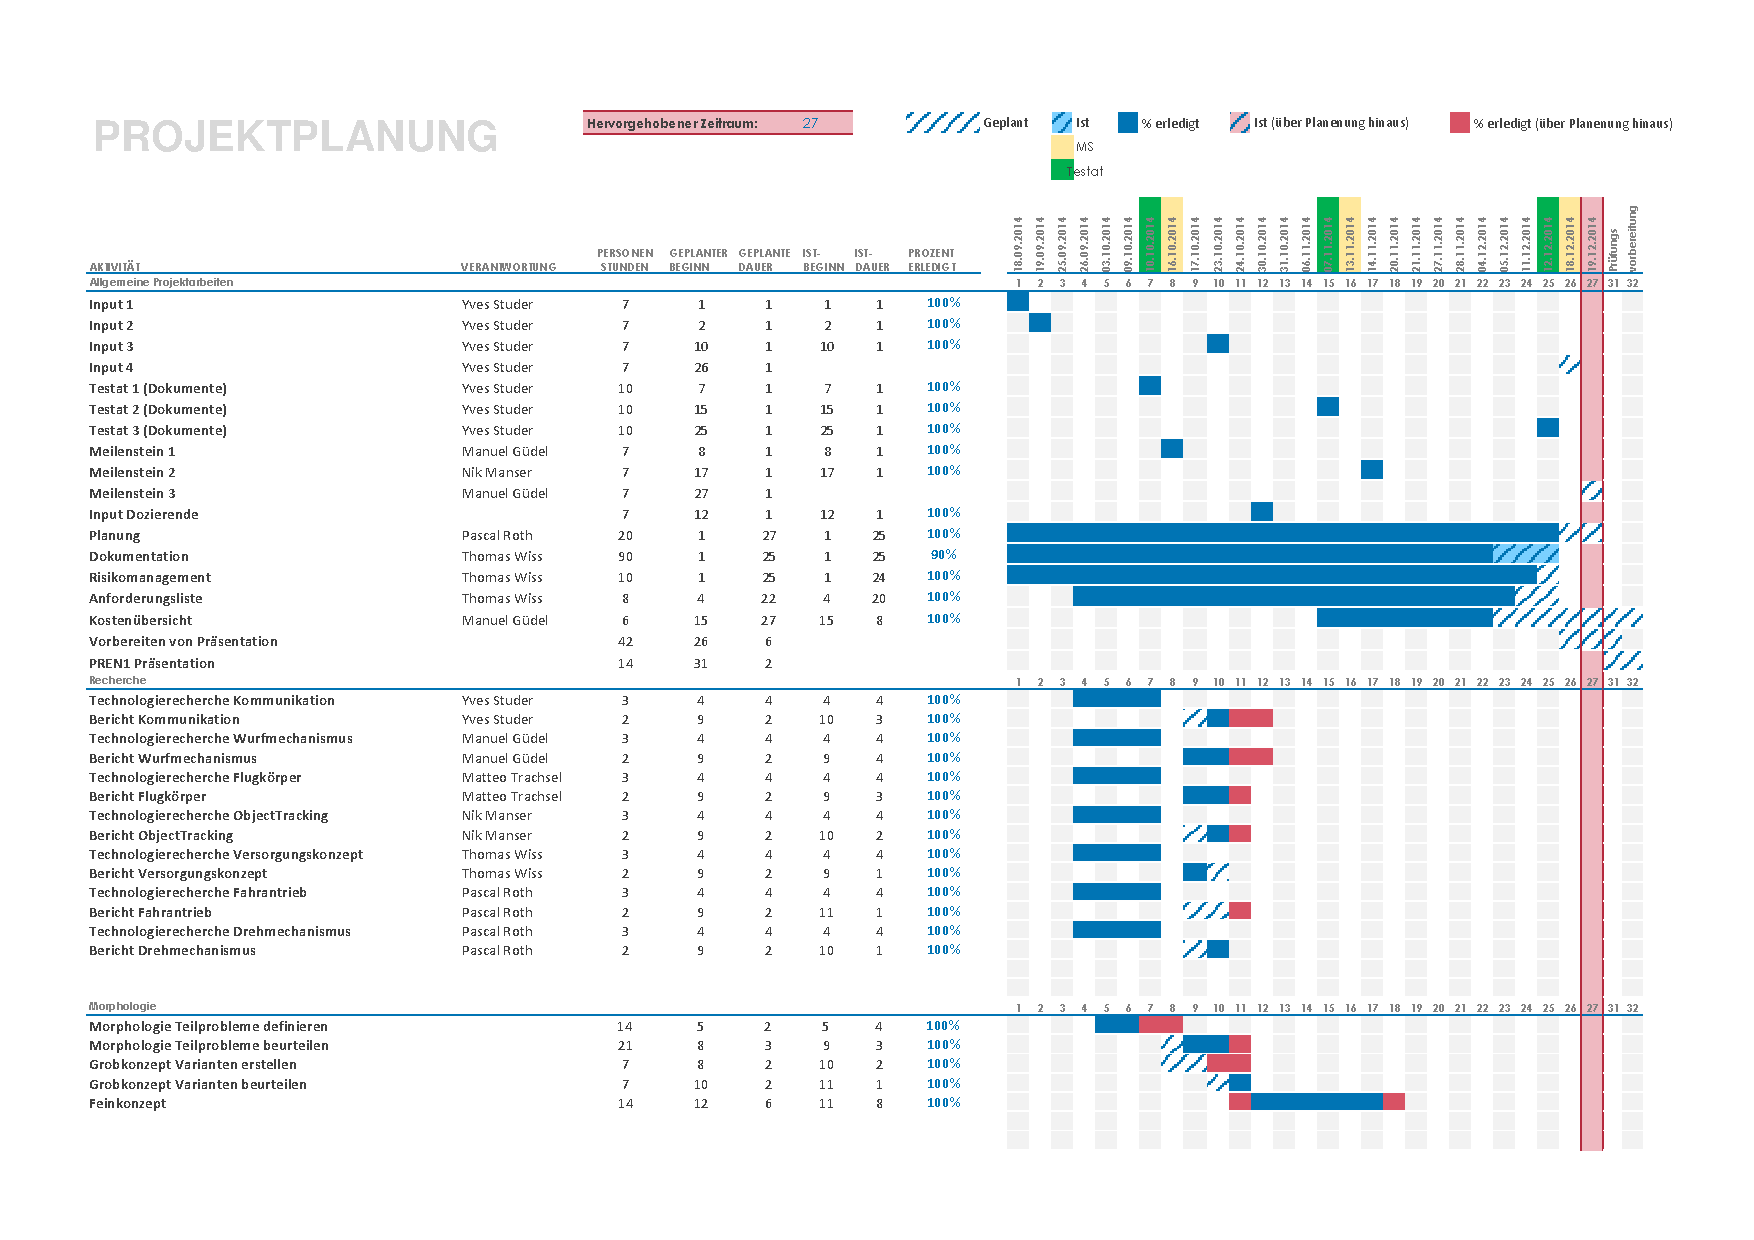
\includegraphics[page=1,scale=0.8,clip,trim=15mm 22mm 13mm 18mm] {Enddokumentation/Projektplanung_Management/Bilder/Projekt-Planung_Team32.pdf}
    \newpage
    \includegraphics[page=2,scale=0.8,clip,trim=15mm 100mm 13mm 10mm] {Enddokumentation/Projektplanung_Management/Bilder/Projekt-Planung_Team32.pdf}
    \newpage
\end{landscape}
\subsubsection{Erläuterung zur Projektplanung}
Um eine grösstmögliche Übersicht zu haben, ist die Projektplanung relativ allgemein gehalten. Das heisst, es sind alle Themen und Arbeitsblöcke vorhanden, jedoch ist nicht jeder einzelne Arbeitsschritt der darin anfällt auch aufgeführt. Ebenso ist pro Arbeitsschritt nur die verantwortliche Person aufgeführt. Sie trägt die Hauptverantwortung über ein Arbeitsblock, jedoch können auch andere Personen daran mitarbeiten. Abgeschlossene und nicht mehr relevante Arbeiten sind nicht aufgeführt.\\
Zeitangaben sind als Schätzungen zu verstehen. Es wurde kein Journal über die geleistete Arbeitszeit geführt.\\
Die auf den vorherigen Seite dargestellte Grafik ist die Projektplanung über den Zeitraum von PREN 1. Arbeiten, die noch nicht fertig sind oder die über den ganzen Zeitraum des PREN-Moduls laufen, werden Ende PREN 1 in eine neue Projektplanung für PREN2 überführt. Für diese Planung wird wiederum die selbe Excel-Vorlage verwendet. 
